\section{Estudio sobre la expresividad de las redes neuronales}

\subsection{Objetivos}
\begin{frame}{Objetivos}
	\begin{itemize}
		\item Estudiar la mayor potencia expresiva de las redes profundas frente a las redes no profundas.
		\item Modelizar una \textbf{tarea de aprendizaje automático}.
		\item Modelizar \textbf{dos tipos de arquitecturas} de aprendizaje automático a partir de ciertas descomposiciones tensoriales.
		      \begin{itemize}
			      \item Arquitectura \textbf{no profunda} o somera, utilizando la descomposición \textit{CP}.
			      \item Arquitectura \textbf{profunda}, empleando la descomposición \textit{HT}.
		      \end{itemize}
		\item Dar dos resultados para estudiar el fenómeno de \textbf{eficiencia en profundidad} y cómo de frecuentemente ocurre.
	\end{itemize}
\end{frame}

\subsection{Tarea de aprendizaje}
\begin{frame}{Tarea de aprendizaje}

	\begin{itemize}
		\item Buscamos resolver una tarea de \textbf{clasificación de imágenes}.
		\item Representamos las imágenes de entrada como \textbf{parches}, $(\nv{x_1}, \ldots, \nv{x_N})$ con $\nv{x_i} \in \R^S$. Esta representación se utiliza en la práctica \cite{matematicas:vit}.
		\item Clasificamos la imagen de entrada como el valor $y$ para el cual se maximiza la \textbf{función de puntuación} $h_y: \R^S \times \cdots \times \R^S \to \R$.
		\item Por lo tanto, buscamos aprender $Y$ funciones de puntuación a partir de los datos y las arquitecturas de aprendizaje automático que desarrollemos.
	\end{itemize}

\end{frame}

\begin{frame}{Función de puntuación}

	\begin{itemize}
		\item \textbf{Funciones de representación} $\conjunto{f_d(\nv{x}): \; d \in \N} \subseteq L^2(\R^S)$. El conjunto de funciones será total y linealmente independiente.
		      \begin{itemize}
			      \item Neuronas.
			      \item \textit{Radial Basis Functions} (Gaussianas).
		      \end{itemize}
		\item Expresamos las combinaciones lineales finitas como:

		      \begin{equation} \label{eq:hipotesis_en_general}
			      h_y(\nv{x_1}, \ldots, \nv{x_N}) \approx \sum_{d_1, \ldots, d_N \in \N} \mathcal{A}^y_{d_1, \ldots, d_N} \prod_{i = 1}^N f_{d_i}(\nv{x_i}).
		      \end{equation}
		\item En \cite{matematicas:principal} se justifica empíricamente que al trabajar con imágenes podemos tomar $M=100$ con lo que se verifica:

		      \begin{equation} \label{eq:puntuacion_general}
			      h_y(\nv{x_1}, \ldots, \nv{x_N}) = \sum_{d_1, \ldots, d_N = 1}^{M} \mathcal{A}^y_{d_1, \ldots, d_N} \prod_{i = 1}^N f_{\theta_{d_i}}(\nv{x_i}).
		      \end{equation}
	\end{itemize}

\end{frame}

\subsection{Modelización de las redes no profundas}
\begin{frame}{Descomposición \textit{CANDECOMP/PARAFAC}}
	\begin{itemize}
		\item Aplicar la descomposición \textit{CP} en el tensor de coeficientes de \eqref{eq:puntuacion_general}.

		      \begin{block}{Descomposición \textit{CANDECOMP/PARAFAC}}
			      Todo tensor $\mathcal{A}$ puede ser expresado como la suma de tensores puros. Es decir, $\forall \mathcal{A} \in \R^{M_1 \times \cdots \times M_N}$, $\exists Z \in \N$:
			      \begin{equation}
				      \mathcal{A} = \sum_{i = 1}^Z \nv{v_i^{(1)}} \otimes \cdots \otimes \nv{v_i^{(N)}};
				      \; \nv{v_i^{(k)}} \in \R^{M_k},
				      \; \forall i \in \deltaset{Z},
				      \; \forall k \in \deltaset{N}.
			      \end{equation}
		      \end{block}
		\item Rango \textit{CP}.
		\item Nuestro modelo queda como:

		      \begin{equation} \label{eq:cp_model}
			      h_y(\nv{x_1}, \ldots, \nv{x_N}) =  \sum_{z = 1}^Z a_z^y \dspace \prod_{i = 1}^N \dspace \sum_{d = 1}^{M} \omega^{z, i}_d \; f_{\theta_{d}}(\nv{x_i}).
		      \end{equation}

	\end{itemize}
\end{frame}

\begin{frame}{Relación con arquitecturas de aprendizaje automático}
	\begin{figure}
		\centering
		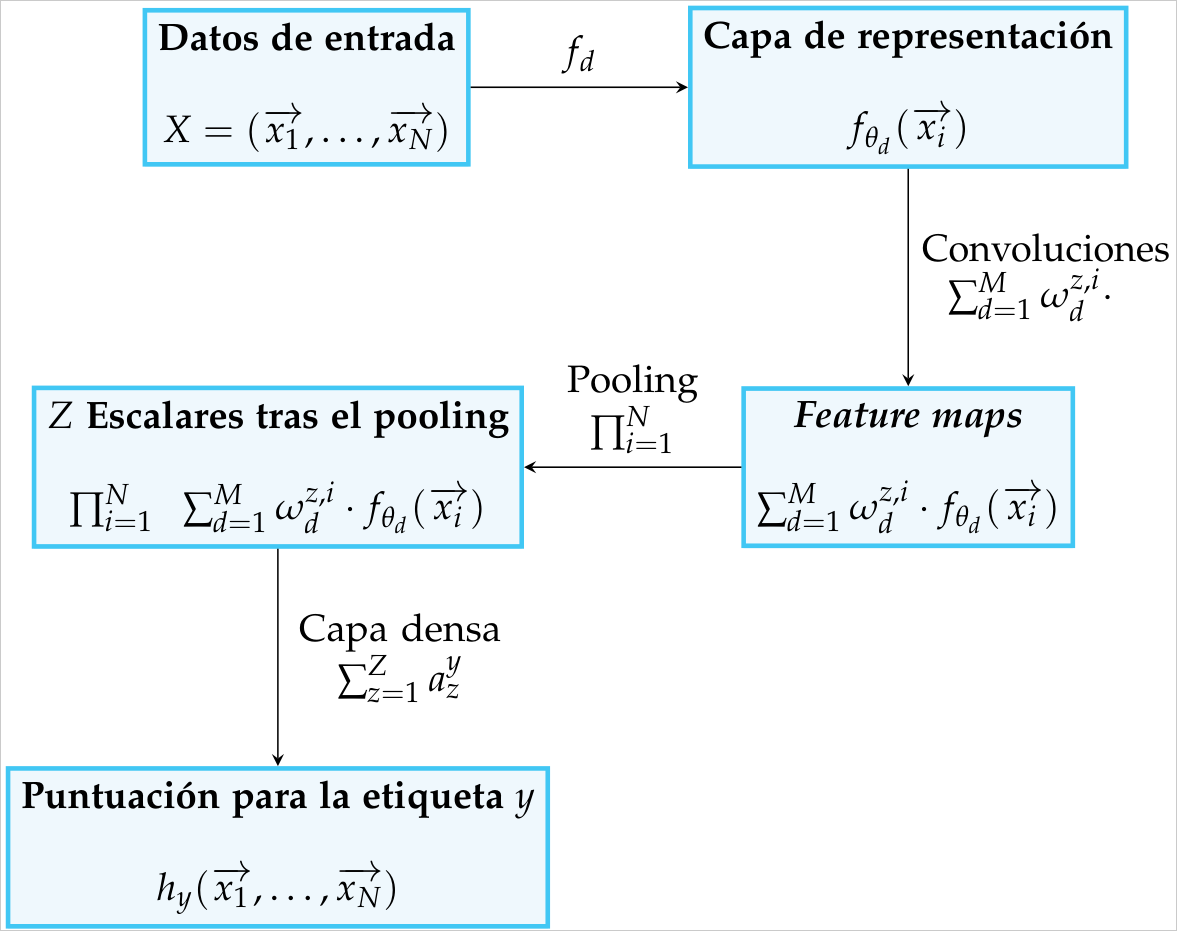
\includegraphics[height=0.9\textheight]{matematicas/relacion_cnn_tikz}
	\end{figure}

\end{frame}


\subsection{Modelización de las redes profundas}
\begin{frame}{Descomposición \textit{Hierarchical \textit{Tucker}}}

	\begin{equation} \label{eq:descomposicion_ht}
		\begin{split}
			\phi^{1, j, \gamma} &:= \sum_{\alpha = 1}^{r_0} a_{\alpha}^{1, j, \gamma} \cdot \nv{\varphi^{2j-1, \alpha}} \otimes \nv{\varphi^{2j, \alpha}} \\
			\ldots \\
			\phi^{l, j, \gamma} &:= \sum_{\alpha = 1}^{r_{l-1}} a_{\alpha}^{l, j, \gamma} \cdot \phi^{l-1, 2j-1, \alpha} \otimes \phi^{l-1, 2j, \alpha} \\
			\ldots \\
			\mathcal{A}^y &:= \sum_{\alpha = 1}^{r_{L-1}} a_{\alpha}^{L, y} \cdot \phi^{L-1, 1, \alpha} \otimes \phi^{L-1, 2, \alpha}
		\end{split}
	\end{equation}

	\begin{itemize}
		\item $l$: nivel en la descomposición.
		\item $j$: posición dentro del nivel $l$.
		\item $\gamma$: tensor de la capa $l$ y posición $j$.
		\item $r_l$: cuántos tensores hay en cada posición $j$ de la capa $l$.
	\end{itemize}

\end{frame}

\begin{frame}{Primer ejemplo}

	\begin{figure}
		\centering
		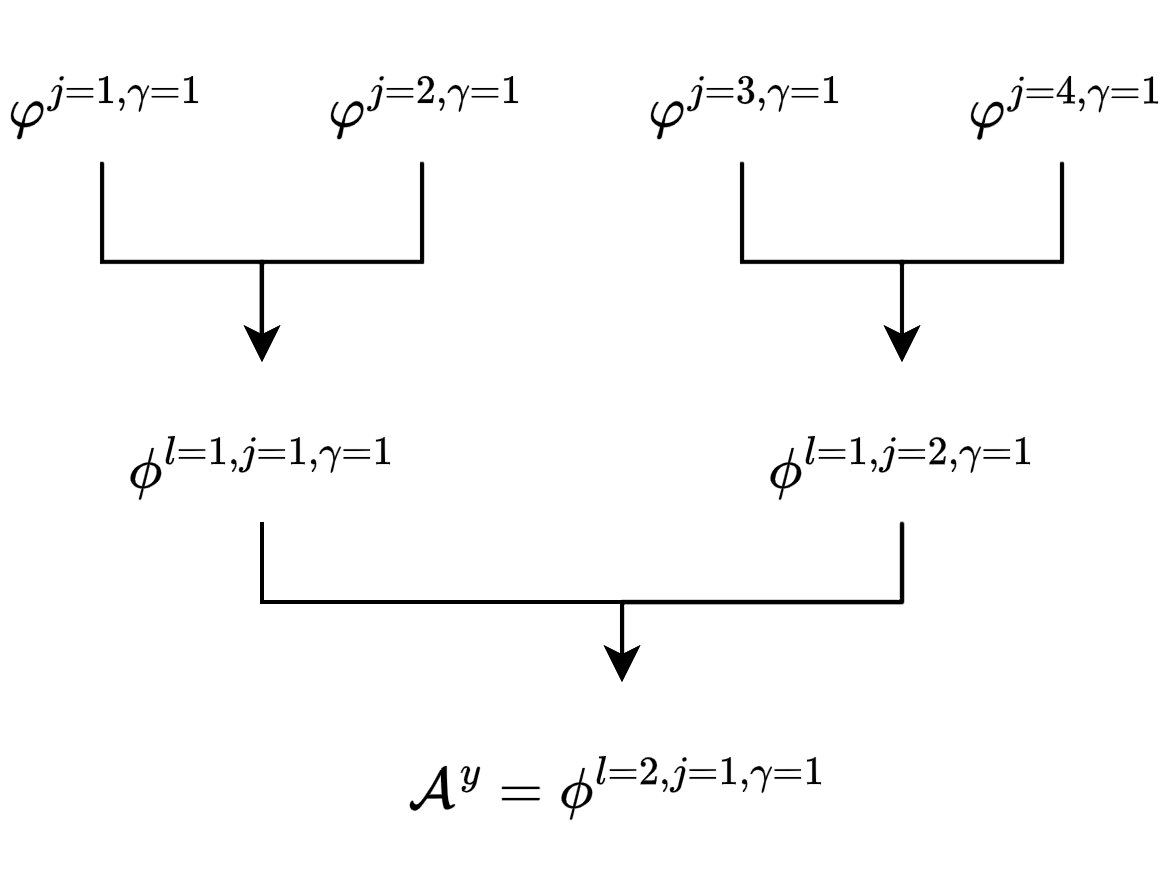
\includegraphics[width=0.7\textwidth]{matematicas/descomp_ht_rank_1}
		\caption{Ejemplo gráfico tomando $r = 1$, $L = 2$.}
		\label{img:diagrama_ht_simple}
	\end{figure}

\end{frame}

\begin{frame}{Segundo ejemplo}

	\begin{figure}
		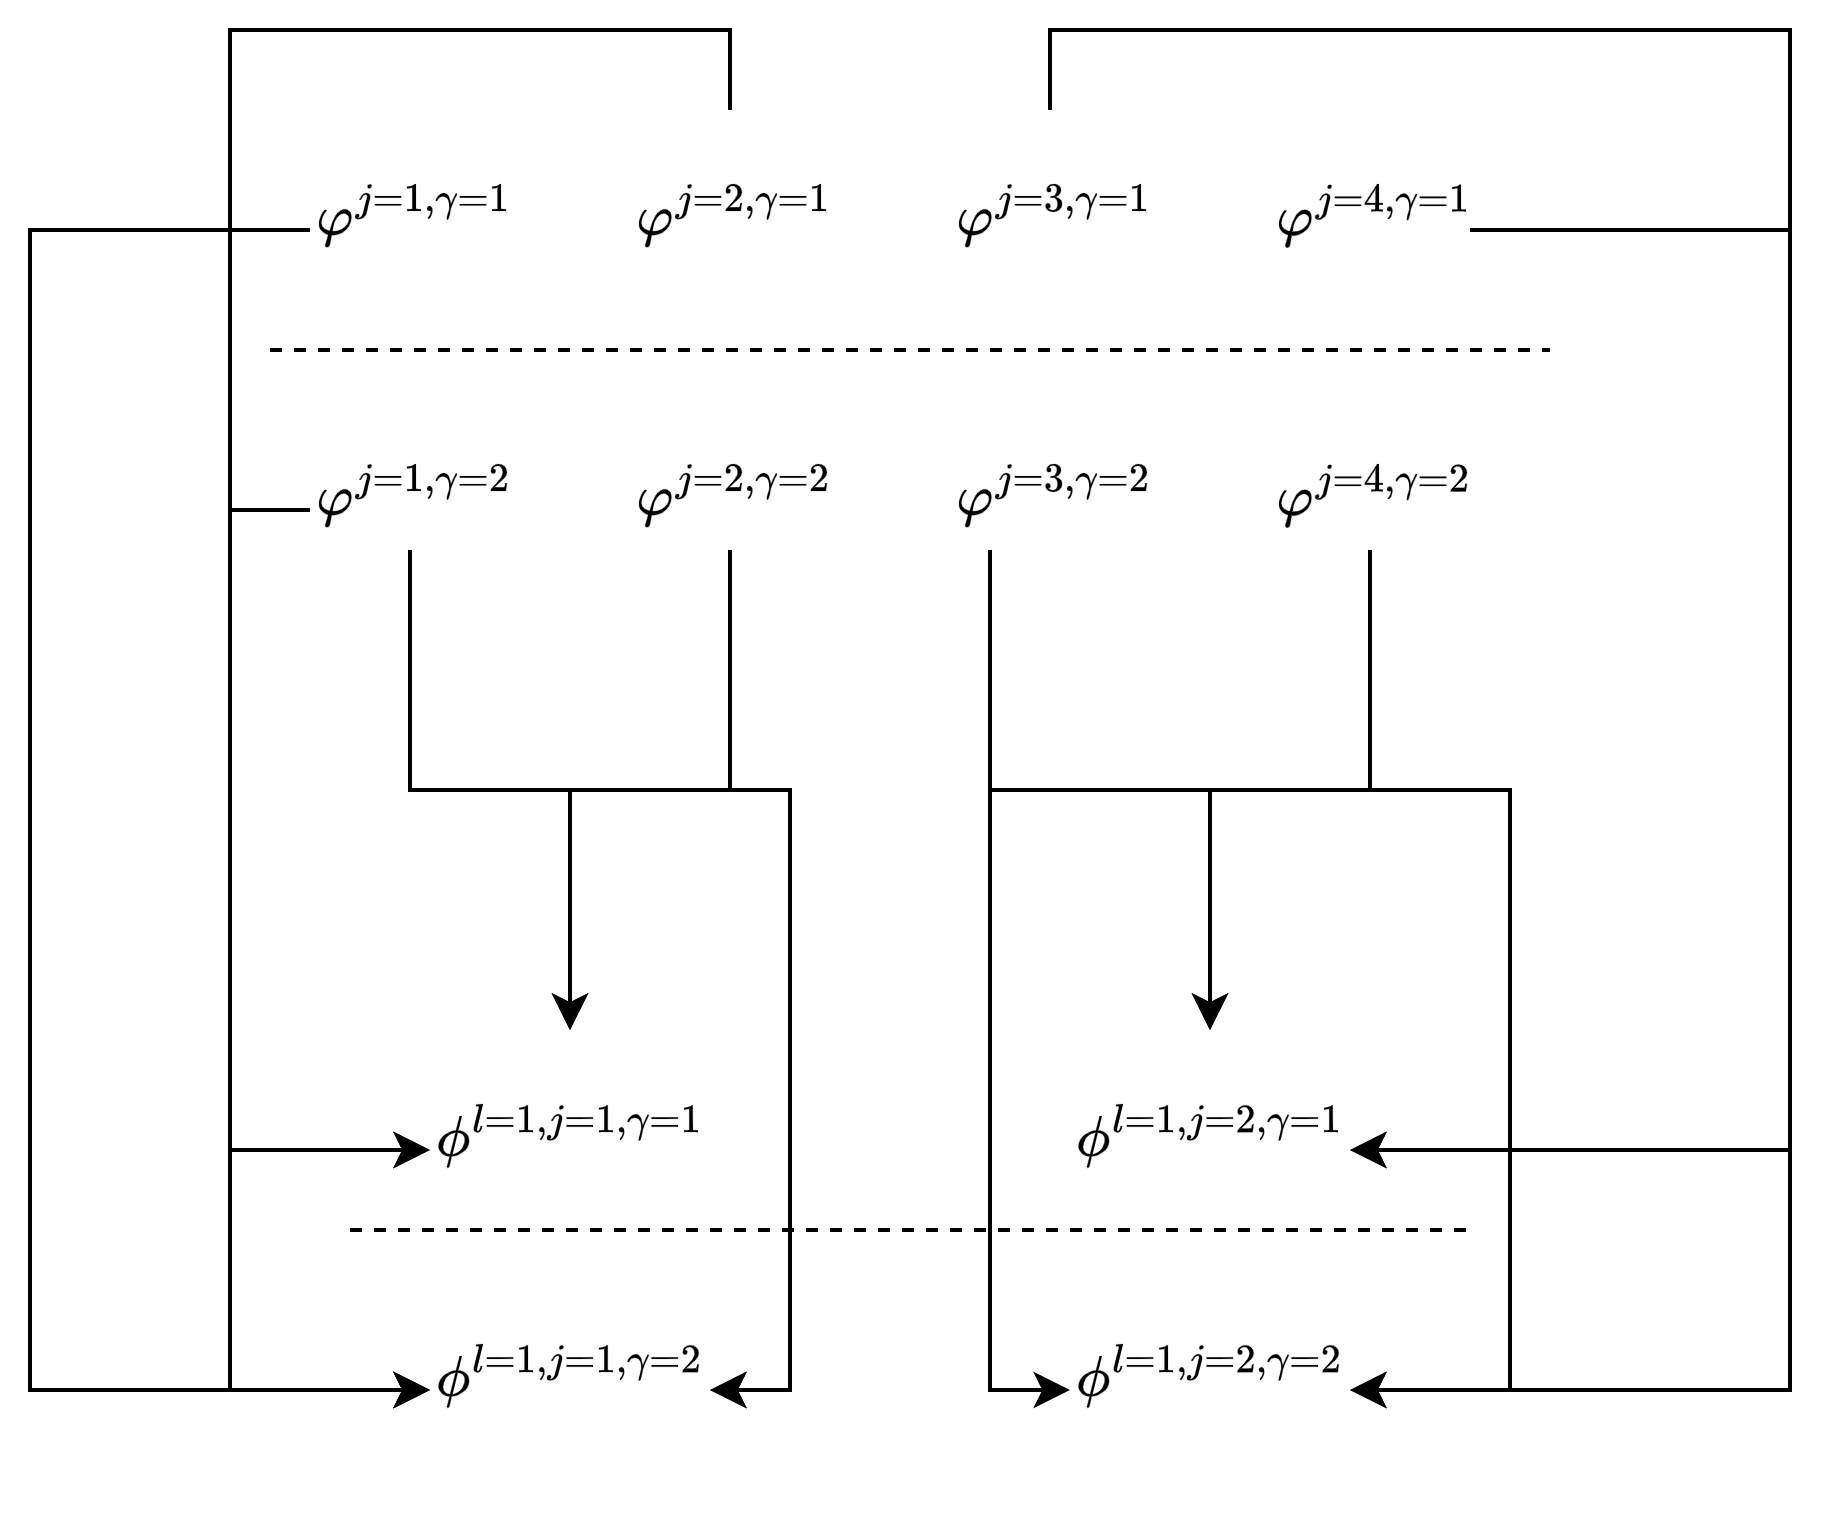
\includegraphics[width=0.7\linewidth]{matematicas/descomp_ht_rank_2_paso_1}
		\caption{Ejemplo gráfico tomando $r = 2$, $L = 2$ capas, primer paso.}
	\end{figure}

\end{frame}

\begin{frame}{Segundo ejemplo}

	\begin{figure}
		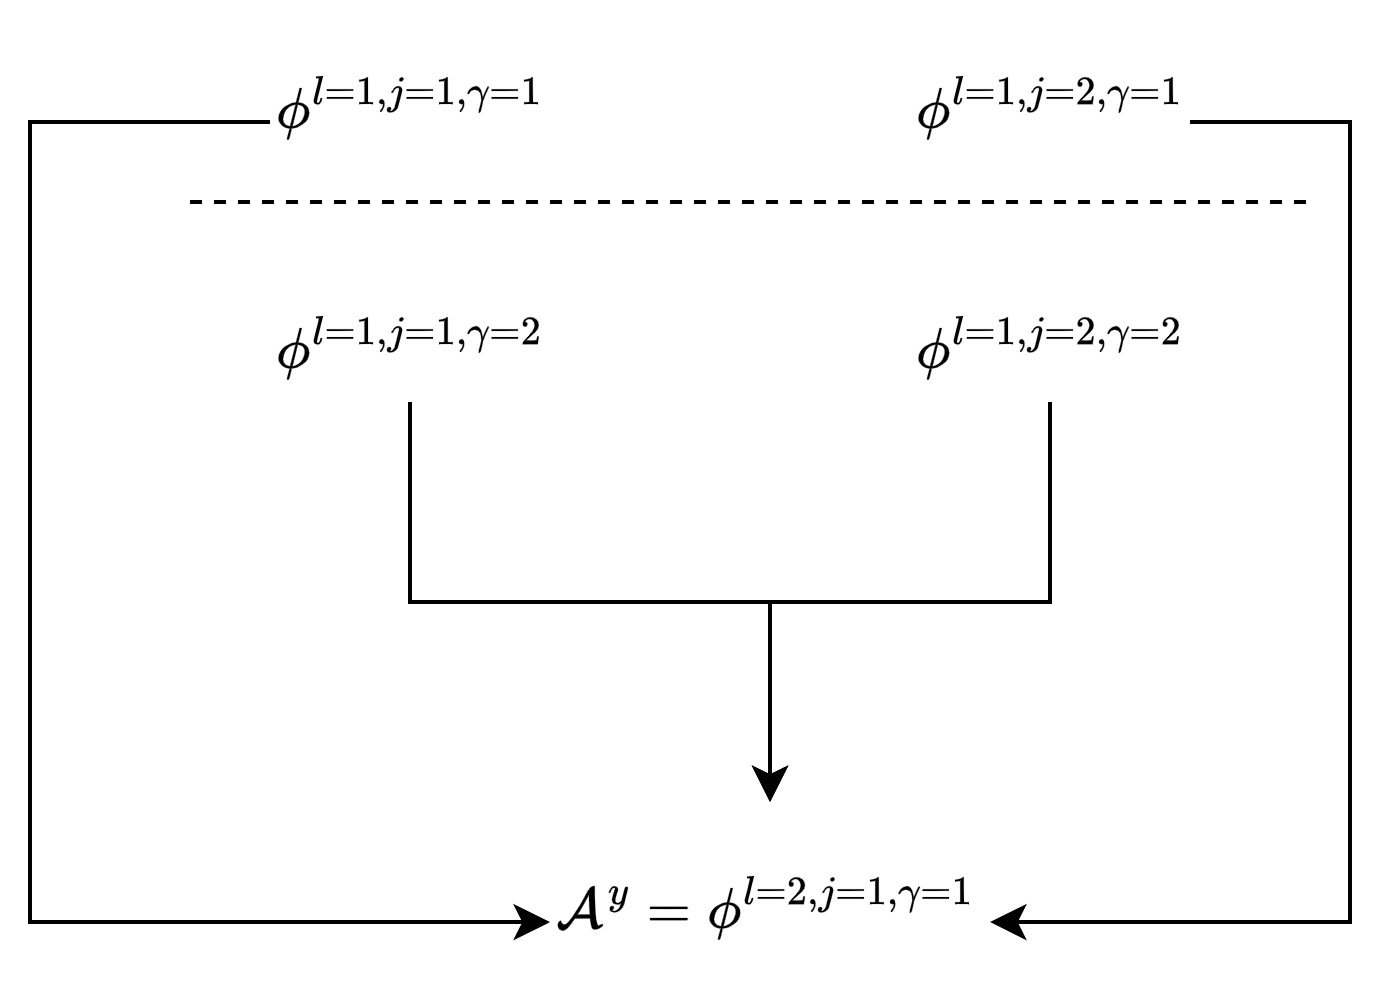
\includegraphics[width=0.7\linewidth]{matematicas/descomp_ht_rank_2_paso_2}
		\caption{Ejemplo gráfico tomando $r = 2$, $L = 2$ capas, segundo paso.}
	\end{figure}

\end{frame}

\begin{frame}{Relación con arquitecturas de aprendizaje automático}

	\begin{figure}
		\centering
		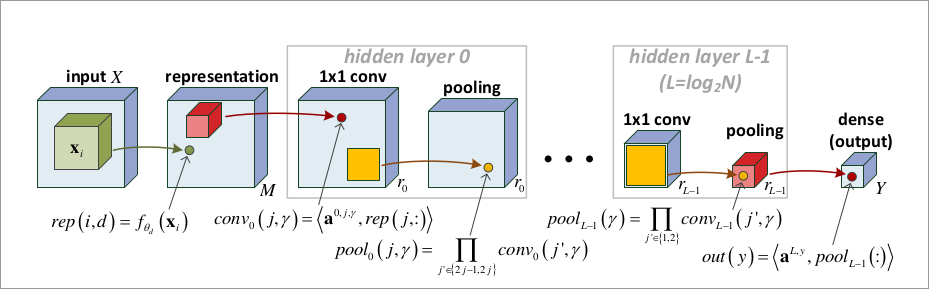
\includegraphics[height=0.42\textheight]{matematicas/diagrama_paper_modelo_ht}
		\caption{Funcionamiento de nuestro modelo. Imagen extraída de \cite{matematicas:principal}.}
	\end{figure}


\end{frame}

\begin{frame}{Eficiencia en profundidad}
	\begin{itemize}
		\item La \textbf{eficiencia en profundidad} es el fenómeno en el que un modelo con un número de parámetros polinomial obtiene una potencia expresiva que en otro modelo require un número exponencial de parámetros.
		      \begin{block}{Penalización en número de parámetros}

			      Dado un tensor $\mathcal{A}^y$ como resultado de un modelo \textit{CP}, realizar dicho tensor con un modelo \textit{HT} requiere de:
			      \begin{equation}
				      N \cdot Z^2 \cdot \frac{2^{L-1} - 1}{2^{L-1}} \encima{\longmapsto}{L \mapsto \infty} N \cdot Z^2.
			      \end{equation}

			      coeficientes adicionales.
		      \end{block}

		\item ¿Y al revés?
	\end{itemize}
\end{frame}

\subsection{Resultados principales}

\begin{frame}{Primer resultado central}

	\begin{block}{Rango \textit{CP} exponencial de un modelo \textit{HT}}
		Sea $\mathcal{A}^y \in \espaciotensores{N}{M}$ dado por las ecuaciones \eqref{eq:descomposicion_ht}. Definamos $r := \min \conjunto{r_0, M}$ y consideremos el espacio de todas las posibles configuraciones de parámetros de nuestro modelo \textit{HT} $\conjunto{ \nv{a^{l, j, \gamma}}}_{l, j, \gamma}$. En este espacio, el tensor generado $\mathcal{A}^y$ tendrá rango \textit{CP} de al menos $r^{N/2}$ casi por doquier. Es decir, el conjunto de parámetros del modelo \textit{HT} con los que el modelo tiene rango \textit{CP} menor que $r^{N/2}$ tiene medida nula. El resultado se mantiene si forzamos los coeficientes compartidos en la ecuación \eqref{eq:descomposicion_ht}. Es decir, haciendo $\nv{a^{l, \gamma}} \equiv \nv{a^{l, j, \gamma}}$ y considerando el espacio de configuraciones $\{ \nv{a^{l, \gamma}}  \}_{l, \gamma}$.

	\end{block}


\end{frame}

\begin{frame}{Segundo resultado central}

	\begin{block}{Incapacidad del modelo \textit{CP} para aproximar eficientemente el modelo \textit{HT}}
		Dado un conjunto de funciones de representación linealmente independientes, $\conjunto{f_{\theta_d}: \; d \in \deltaset{M}}$, aleatorizar los pesos de un modelo \textit{HT} \eqref{eq:descomposicion_ht} a partir de una distribución de probabilidad continua induce funciones de puntuación $h_y$ que con probabilidad uno no pueden ser aproximadas arbitrariamente bien (en el sentido $L^2$) por un modelo \textit{CP} con un valor de $r$ menor que $r := \min \{r_0, M \}^{N/2}$. Este resultado se mantiene forzando los coeficientes compartidos en el modelo \textit{HT} mientras que dejamos el modelo \textit{CP} sin restricciones.
	\end{block}

\end{frame}

\begin{frame}{Conclusiones}
	\begin{itemize}
		\item Hemos modelado la tarea de aprendizaje y los dos tipos de arquitectura, profunda y no profunda.
		\item El primer resultado nos dice que casi todos los tensores $\mathcal{A}^y$ que podemos generar con un modelo \textit{HT} tienen rango \textit{CP} de al menos $r^{N/2}$, lo que implica que el modelo \textit{CP} necesita un número exponencial de parámetros.
		\item El segundo resultado añade a este hecho que ni siquiera pueden aproximarse eficientemente (menos de un número exponencial de coeficientes) por una descomposición \textit{CP}.
		\item Hemos dado información precisa sobre cómo de frecuente ocurre este hecho (casi por doquier). Otros trabajos \cite{matematicas:descomposicion_ht} únicamente dan ejemplos concretos en los que esto ocurre.
	\end{itemize}
\end{frame}
